\setchapterpreamble[u]{\margintoc}
\glsresetall % reset glossary
\chapter{Optimizing the layout of the modules in space}
Chapter~\ref{05} introduced the basic concept of modular structures and  . Additionally it conducted a design of experiments that helped us undertanddig the general mechanical behaviour of modular stuctures. However we saw that expecially the volume of such structure is very penalyzed if the structure is 


\section{Optimize the modules' layout using a modified DMO algorithm}
The objective of this study is to address the concurrent optimization of both the layout and topology of multiple modules within a modular structure. The key scientific challenge lies in the discrete nature of the layout optimization problem \ie find the optimal distribuition of the different modules within the subdomains of the structure, an inherently discrete problem. Given our intent to employ a gradient descent algorithm \sidecite{sigmund_usefulness_2011}, it is imperative to design a methodology for converting the discrete nature of the problem into a continuous one, permitting the application of gradient-based optimization techniques.

\subsection{Definition of the subdomains cross-sectional areas}
In this study, our strategy for addressing the discrete layout problem of modules as a continuous one involves defining the variables of the subdomains (i.e., the structure's variables) as a weighted sum of the module variables. This approach draws inspiration from the seminal work of Stegmann and Lund in the \gls{dmo} algorithm \sidecite{stegmann_discrete_2005}, where an optimizer selects the optimal homogenized stiffness tensor for each subdomain from a set of fixed tensors to minimize the compliance of a given structure. In the scenario of discretizing a ground structure into $N_\text{sub}$ subdomains and utilizing $N_\text{T}$ distinct modules, the cross-sectional areas of subdomain $j$ are then expressed as:  
\begin{equation}
    \vect{a}^j = \sum_{t=1}^{N_\text{T}} w_t^j \bar{\vect{a}}_t 
\end{equation}
where $\bar{\vect{a}}_t $ represent the vector of cross-sectional areas of the t module and $\vect{w}^j$ is the vector of weight relatives to the $j$ subdomain, defined as $ \vect{w}^j \in \mathbb{R}^t\,|\,w_j^t \in [0,1]$.

An example of a cantilever beam with $N_\text{sub}=8$ and $N_\text{T}=$ is illustrated in \figref{fig:06_weighted_sum}, in which we visually demonstrate the impact of modifying the weight values $w$ on the structure topology.

\begin{figure*}
    \centering
    \includegraphics{figures/06_DMO/00_weight_dmo/weight_dmo.pdf}
    \caption{}
    \label{fig:06_weighted_sum}
\end{figure*}

\subsection{Variables penalization schemes}
The inherent limitation of the proposed approach is that, when the optimizer converges to a solution, the weights of all subdomains must converge to either zero or one, with the additional constraint that only one weight per subdomain can be equal to one. This is necessary to avoid intermediate weights, which would imply a combination of multiple modules' topologies lacking mechanical significance and proving impractical for manufacturing. To address this issue, we implement an interpolation scheme that penalizes intermediate weights. Specifically, we opt for the \gls{ramp} method \sidecite{stolpe_alternative_2001} instead of the more commonly used \gls{simp} interpolation scheme. This choice is motivated by \gls{ramp}'s advantageous property of ensuring that the derivative is never infinite nor zero when approaching a value of zero.

We define the design variable $\matr{\alpha}\in\mathbb{R}^{j,t}$ as the modules' layout variable, responsible for the module choice within the subdomain $j$. Its relationship with the weight $w$ is as follows:
\begin{equation}
    w_t^j = \frac{\alpha_t^j}{1+p(1-\alpha_t^j)}    
\end{equation}
where $p \in \mathbb{R}^+$ denotes a parameter governing the steepness of the \gls{ramp} interpolation. Drawing inspiration from the works of \sidecite{hvejsel_material_2011}, we introduce a multi-phase variant of the \gls{ramp} interpolation, in which we concurrently penalize mechanical properties while artificially increasing the volume of modules with intermediate densities. To achieve this, we introduce an additional \gls{ramp} parameter, $q$, always negative ($q \in \mathbb{R}^-$), utilized to assess the augmented weights associated with the volume evaluation $V$. We can then write:
\begin{equation}
    V = \sum_{j=1}^{N_{\text{sub}}}\vect{\bar{\ell}}^T\tilde{\vect{a}}^j,
\end{equation}
where the vector $\tilde{\vect{a}}^j$, representing the increases scross-sectional areas of the $j$-th subdomain is defined as following:
\begin{equation}
    \tilde{\vect{a}}^j = \sum_{t=1}^{N_\text{T}} \tilde{w}_t^j \bar{\vect{a}}_t, 
\end{equation}
and where $\tilde{w}$ is:
\begin{equation}
    \tilde{w}_t^j = \frac{\alpha_t^j}{1+q(1-\alpha_t^j)}.    
\end{equation}
So for every design variable $\alpha$, we associate two different weights ($w$ and $\tilde{w}$) that are used to evaluate the mechanical properties and the structure volume, respectively (see \figref{fig:06_ramp}).


\begin{figure}
    \centering
    \includegraphics{figures/06_DMO/00_ramp/ramp.pdf}
    \caption{}
    \label{fig:06_ramp}
\end{figure}

\subsection{The optimization formulation and resolution algorithm}
The objective function of the optimization process is the volume minimization of the modular structure. The members of the structure are subject to multiple mechanical constraints, namely stress, topological buckling, minimum slenderness, and compatibility constraints. Formulation $\mathbb{M}_1$ is stated in terms of modules' cross-sectional area $\bar{\vect{a}}$, module selection variables $\vect{\alpha}$, member forces $\vect{q}$, and nodal displacements $\vect{U}$ as follows:
\begin{equation}
    \begin{aligned}
    \min_{\bar{\vect{a}}, \vect{\alpha}, \bm{q}, \bm{U}}   && V &= \sum_{j=1}^{N_{\text{sub}}}\vect{\bar{\ell}}^T\tilde{\vect{a}}^j && \textrm{(Volume minimization)}\\
    \textrm{s.t.}   && \bm{B}\bm{q} &= \bm{f} && \textrm{(Force equilibrium)}\\
                    && \bm{q} &= \frac{\bm{a}\bm{E}}{\bm{\ell}}\bm{b}^T\bm{U} && \textrm{(Compatibility constraints)} \\
                    && \bm{q} &\geq -\frac{\bm{s}\bm{a}^2}{\bm{\ell^2}} && \textrm{(Euler buckling constraints)} \\
                    && -\sigma_C\bm{a} &\leq \bm{q} \leq \sigma_T\bm{a} && \textrm{(Stress constraints)} \\
                    && \bar{\vect{a}}_{t,r}&\geq \bar{a}_{t,r=1} && r \in \mathcal{C}_{l,r}(\bar{\vect{a}}_t),\, \forall t \\
                    && 0 &\leq \bar{\vect{a}} \leq \frac{4 \pi \bar{\vect{\ell}}^2}{\lambda_{\text{max}}} && \textrm{(Slenderness limit)} \\
                    && \sum_{t=1}^{N_\text{T}} \alpha_t^j &\leq 1, \; \forall j && \textrm{(One selected module max.)} \\
    \end{aligned}
    \tag{$\mathbb{M}_1$}
    \label{eq:06_optim_complete}
\end{equation}

This formulation builds on the classic \gls{dmo} approach, adding multiple mechanical constraints and while operating on a ground structure. Additionally, we are not only selecting the best module for every subdomain by changing the value of $\alpha$ as classic \gls{dmo} does, but we are also optimizing the modules' topology simultaneously. This simultaneous optimization presents a more challenging task. The advantages of this formulation lie in dealing with a discrete problem using continuous design variables and a gradient-based optimizer. However, it comes with the drawback of increasing the problem size, as we are adding numerous additional design variables $\alpha$ that scale with the number of subdomains and the number of modules \ie a vector of size $\vect{\alpha}^j \in \mathbb{R}^t$ is defined for every one of the $j$ subdomains.

The design variables $\alpha$ are constrained by a set of constraints that limit the maximum sum of $\alpha$ of a submodule $j$ to be less than or equal to one. It is crucial to note that we treat this constraint as a disequality constraint rather than an equality. This allows the optimizer to set all $\alpha$ to zero, permitting the removal of the subdomain from the structure. The constraint is expressed as follows:
\begin{equation}
    \sum_{t=1}^{N_\text{T}} \alpha_t^j \leq 1, \; \forall j 
\end{equation}

Problem \eqrefnotext{eq:06_optim_complete} is tackled using a modified version of the proposed two-step solving algorithm. In this approach, we initially solve a relaxed problem denoted as $\mathbb{M}_2$, where kinematic compatibility constraints are omitted. This relaxed problem is inherently nonlinear due to the introduction of the $\alpha$ design variables. For this iteration, we have chosen to solve it in this form without linearizing the buckling constraints.

The relaxed formulation $\mathbb{M}_2$, expressed in terms of modules' cross-sectional area $\bar{\vect{a}}$, module selection variables $\vect{\alpha}$, and member forces $\vect{q}$, is the following:
\begin{equation}
    \begin{aligned}
    \min_{\bar{\vect{a}}, \vect{\alpha}, \bm{q}}   && V &= \sum_{j=1}^{N_{\text{sub}}}\vect{\bar{\ell}}^T\tilde{\vect{a}}^j && \textrm{(Volume minimization)}\\
    \textrm{s.t.}   && \bm{B}\bm{q} &= \bm{f} && \textrm{(Force equilibrium)}\\
                    && \bm{q} &\geq -\frac{\bm{s}\bm{a}^2}{\bm{\ell^2}} && \textrm{(Euler buckling constraints)} \\
                    && -\sigma_C\bm{a} &\leq \bm{q} \leq \sigma_T\bm{a} && \textrm{(Stress constraints)} \\
                    && 0 &\leq \bar{\vect{a}} \leq \frac{4 \pi \bar{\vect{\ell}}^2}{\lambda_{\text{max}}} && \textrm{(Slenderness limit)} \\
                    && \sum_{t=1}^{N_\text{T}} \alpha_t^j &\leq 1, \; \forall j && \textrm{(One selected module max.)} \\
    \end{aligned}
    \tag{$\mathbb{M}_2$}
    \label{eq:06_optim_relax}
\end{equation}
Problem $\mathbb{M}_2$ is solved using a non-linear gradient-based optimizer that iteratively exploits first and second-order derivatives to achieve convergence. The computation of the Jacobian and Hessian matrices for this problem is not trivial, and the details are elaborated in \appref{app:01}.

Once problem $\mathbb{M}_2$ is solved, we perepare for the second step in wich the kinematic compatibility constraints are added again. We exploit the optimized module layout $\vect{\alpha}^*$ to set up the fixed module layout on the structure, and evaluate the mapping matrix $H$ used in the variable linking approach of problem ${\mathbb{M}}_\text{1,VL}$. The indexes of the mapping matrix $H$ are evaluated as follows:
\begin{equation}
    h_{j,t} =
    \begin{cases}
      1 & \text{if $\alpha^*_{j,t} = \max(\vect{\alpha}^*_{j})$ and $\alpha^*_{j,t}>0.01$} \\
      0 & \text{otherwise.} 
    \end{cases}
\end{equation}
Subsequently, the compatibility constraints are reintroduced, and a \gls{fea} is conducted to evaluate the displacements $\vect{U}$ used in the starting point of the following optimization step. To mitigate the risk of becoming trapped in local minima, the second step is solved on a reduced design space. The solution $\vect{\bar{a}}^*$ of the first optimization is used to simplifying the initial ground structure, thereby eliminating elements from the optimization that fall below the specified threshold value $a_{\text{thr}}$:
\begin{equation}
    \bar{a}_i<a_{\text{thr}} \; \forall i, \text{ with }a_{\text{thr}} = \chi \; \max(\bar{\vect{a}}^*),
    \label{eq:06_thr}
\end{equation}
with the parameter $\chi$ is the cross-sectional area threshold value.

Now, with all the components in place, we can set up the variable linking formulation ${\mathbb{M}}_{1,\text{VL}}$, as defined in Chapter~\ref{chap:05}. This formulation is employed to optimize modular structures with a fixed modules' layout and provide the final optimized design.
\marginnote{Formulation ${\mathbb{M}}_\text{1,VL}$, defined in Chapter~\ref{chap:05} permits to optimize modular structures with fixed module layout using the variable linking approach. It is stated in terms of modular cross-sectional areas $\bar{\vect{a}}$, member forces $\vect{q}$ and nodal displacements $\vect{U}$ as follows:
\begin{equation*}
    \begin{aligned}
    \min_{\bar{\vect{a}}, \vect{q}, \vect{U}}   && V &= \vect{\ell}^{T}\vect{a}\\
    \textrm{s.t.}  && \vect{a} &= \sum_{t=1}^{N_\text{T}} \vect{h}_t\otimes\bar{\vect{a}}_t \\ 
    && \matr{B}\vect{q} &= \vect{f} && \\
    && \vect{q} &= \frac{\vect{a}E}{\vect{\ell}}\vect{b}^T\vect{U} &&  \\
    && \vect{q} &\geq -\frac{s\vect{a}^2}{\vect{\ell}^{*2}} &&  \\
    && -\sigma_c\vect{a} &\leq \vect{q} \leq \sigma_t\vect{a} &&  \\
    && \bar{\vect{a}}_{t,r}&\geq \bar{a}_{t,r=1}\\
    && 0 &\leq \bar{\vect{a}} \leq \frac{4 \pi \bar{\vect{\ell}}^2}{\lambda_{\text{max}}}, \\
    \end{aligned}
\end{equation*}
}
\subsection{Optimization initialization: a clustering algorithm to identify similarly behaving subdomains}
In the proposed optimization formulation, we not only adjust the design variables responsible for the modules' layout ($\vect{\alpha}$) but also optimize the modules' topology $(\bar{\vect{a}}$). However, a significant challenge arises in this problem due to the strong interdependence between the layout and the module topology \ie the topology of the module is optimized in function of the layout and \textit{vice versatile}. It becomes particularly challenging for a gradient-based optimizer to determine the appropriate direction to follow, especially when starting from a completely uniform initial point (as observed in the work of \sidecite{bakker_simultaneous_2021}). To mitigate this challenge, we provide a slightly influenced starting point for the optimization process. In this work, we influence the module topology design variable at iteration zero $\vect{\alpha}_\text{it}=0$ as follows:
\begin{equation}
    \alpha_{t,\text{init}}^j =
    \begin{cases}
        \frac{1}{N_\text{T}} \cdot 1.1  & \text{if the $j$-th subdomain has the $t$-th module selected,}\\
        \frac{N_\text{T} - 1.1}{N_\text{T}(N_\text{T} - 1)} & \text{otherwise.} \\
    \end{cases}  
\end{equation}

\begin{figure*}
    \centering
    \includegraphics{figures/06_DMO/00_stress_clustering/stress_clustering.pdf}
    \caption{}
    \label{fig:06_kmeans}
\end{figure*}

\begin{figure*}
    \centering
    \includegraphics{figures/06_DMO/00_x0/x0.pdf}
    \caption{}
    \label{fig:06_x0}
\end{figure*}

The idea behind how to select the best module for a subdomain is to identify subdomains that show similar mechanical behavior, grouping them based on their stress state. This grouping is assessed using a k-means clustering technique with the number of clusters equal to the number of module topologies, $N_\text{T}$. Given a set of observations $(x_1, x_2, ..., x_{N_\text{sub}})$, where each observation is a $\bar{n}$-dimensional real vector, k-means clustering aims to partition the $N_\text{sub}$ observations into $N_\text{T}$ sets. In our context, each observation is the vector containing the \acrfull{fea} calculated stress distribution on the initial ground structure with a uniform cross-sectional area.

Additionally, besides the $\bar{n}$ stress values, we introduce the stress state $S$ for the $j$-th submodule as:
\begin{equation}
    S^j = \sum_{i=0}^{\bar{n}}|\sigma_i^j|
\end{equation}
This addition promotes the clustering not only of submodules loaded in similar ways but also based on similar magnitudes, thereby accounting for variations in voluminous and less voluminous modules.

The full clustering process is depicted in \figref{fig:06_kmeans}, showcasing how the grouping is conducted from the same starting point (FEA-calculated stress distribution on the uniform initial ground structure) but with different numbers of clusters ($N_\text{T}=2$, 3, and 5). Finally, \figref{fig:06_x0} illustrates the initial starting point of the optimization, with a uniform initialization of $\bar{a}$ and the biased weight distribution based on the k-means clustering.

\section{Numerical application}\label{sec:06_num_app}
\todo{start from here}
All of the examples presented in this section are solved using the proposed two step formulation, where in the first step we solve a relaxed formulation (no compatibility constraints) to find the optimized modules layout and topology. later, the layout of the modules is fixed, and we solve the optimization problem again to force the structure to comply with the compatibility constraints. The formulations are solved using the non liner interior point solver IPOPT for the two optimization steps 

A continuation scheme is set up on the penalization parameter $q$ of the RAMp interpolation scheme used to evaluate the subdomain volume, where the parameter is set up at zero, and then it increase to -0.4 and -0.8 every time the (and the optimizer is not in a restoration phase). The continaution scgheme is implemented only on $q$ as IPOPT is an interior point algorithm, and increasing the $p$ parameter would put the optimizer well outside of the fesable region everi time the parameter every time it is increased, creating a less than ideal situation. the parameter $\chi$ called the cross-sectional area threshold value is set to 1e-4

The stopping criterion used for the \gls{nlp} optimizations is $\norm{\Delta_{\text{NLP}}}_\infty \leq \text{tol}_{nlp}$, with and $\text{tol}_{nlp}=10^{-8}$. $\Delta_{\text{NLP}}$ represents the scaled \gls{nlp} error, a more comprehensive value used by IPOPT to take into account the optimality of the solution and the constraints violation. The objective function is always scaled so that the initial volume is 1000, the areas are in the interval $[0,100]$, the initial forces in $[0,100]$, and the displacement in $[0,100]$ for the \gls{nlp}. Several additional parameters are used in the \gls{nlp} step for cyipopt and IPOPT:
\begin{itemize}
    \item \texttt{mu\_strategy} is set to \texttt{adaptive} 
    \item \texttt{jac\_c\_constant} is set to \texttt{yes} 
    \item \texttt{num\_linear\_variables} is set to \texttt{N}, with $N$ equal to the number of bars as the force is linear in this problem
    \item \texttt{grad\_f\_constant} is set to \texttt{yes} 
    \item \texttt{linear\_solver} is set to \texttt{pardiso}
    \item \texttt{bound\_push} is set to \texttt{1e-12}
    \item \texttt{constr\_viol\_tol} is set to \texttt{1e-6}
    \item \texttt{nlp\_scaling\_method} is set to \texttt{user-scaling}.
\end{itemize}

\subsection{Layout optimization of fixed modules}
\begin{marginfigure}
    \centering
    \includegraphics[width=\linewidth]{figures/06_DMO/00_cantilever_bcs/cant_mesh.pdf}
    \caption{Boundary conditions of the 2D cantilever beam divided in 24x12 subdomains. In the upper part of the image the ground structure of the module composed of $\bar{n}=6$ elements.}
    \label{fig:06_cant_BC_GS}
\end{marginfigure}
The proposed formulation is very versatile and permits to solve very different optimization problem. We start now by optimizing the most simple we can for modular structures.we want to optimize the distribution of a fixed topology cell inside a given domain, and the optimizer should only chose between having the subdomain poupulated or not. We take a single module topology that is held fixed during the optimization, so nt=1 and $\bar{a}_i=0.6,\,\forall i$. The only degree of fredoom given to the optimizer is the value of the weight w controlled by the design variable $\alpha$.

The structure that is optimized is a two dimensional cantilever beam of dimension $200x100$ with a center load of magnitude $P=1$. The optimization domain is partitioned into $24x12$ submodules on the x and y axis, respectively. Every subdomain is poupulated with a simple fully connected $2x2$ nodes ground structure with 6 candidate bars as shown in \figref{fig:06_cant_BC_GS} The units of the test case are normalized and a list of the geometry and material parameters is given in \tabref{tab:06_modular_cant_data}. Additionally, in these examples buckling and compatibility constraints are relaxed for simplicity and to preserve the solution simmetry.

\begin{margintable}
    \small
    \centering
    \begin{tabular}{cc}
    \toprule
    \textbf{Parameter}        & \textbf{Value} \\ \midrule
    $L$              & 100     \\
    $\sigma_\text{c}, \sigma_\text{t}$ & $\pm 1$\\
    $P$              & 1   \\
    $a_\text{max}$              & 0.6   \\
    \bottomrule
    \end{tabular}
    \caption{Material data used for the 2D cantilever beam 2D.}
    \label{tab:06_modular_cant_data}
\end{margintable}

Before showing and commenting the optimization results, we presents two boundary cases that allow us to better understund and put into perspective the optimization results. first, we set up a monolithic optimization with no modular constraints and setting a maximum cross sectional area $a_\text{max}=0.6$. The optimization is performed on the same ground structure shown in \figref{fig:06_cant_BC_GS}. This results shold represent the lower bound of the optimization, representing the minimum value at wich modular optimization should tend, the closest to this value, the better. The resulting topology shows a volume $V=832.848$ and a thopology that ressembles the one that are obtained in classic topology optimization. Secondly, a we present a fully modular structure, in which all the subdomains presrnt the topology of the fixed topology module with all bars set to 0.6. In that case the structure shows a volume $V=9832.935$ and it represent the upper bound for the optimization. The topology of the fully modular structure is shown in \figref{fig:06_cant_BC_cell}.

\begin{marginfigure}
    \centering
    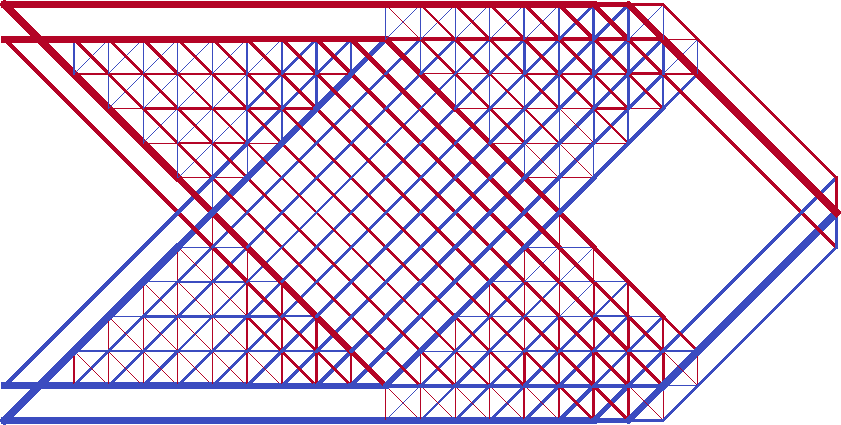
\includegraphics[width=\linewidth]{figures/06_DMO/00_cantilever_extremes/mono.pdf}
    \caption{$V=832.848$}
    \label{fig:06_cant_mono}
\end{marginfigure}


\begin{marginfigure}
    \centering
    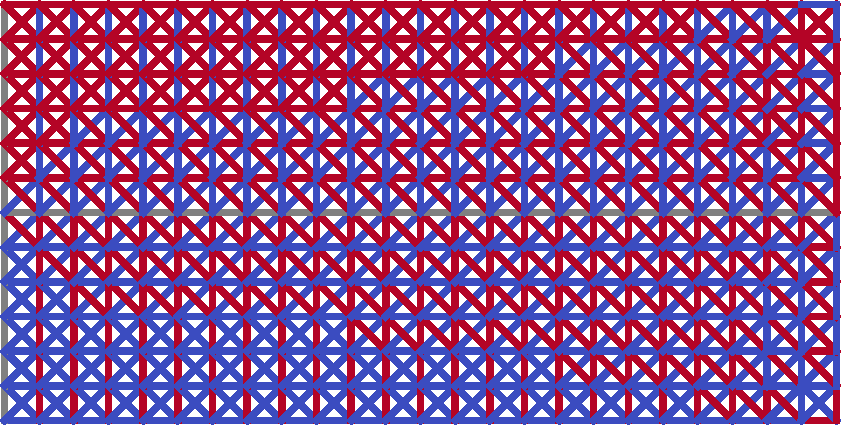
\includegraphics[width=\linewidth]{figures/06_DMO/00_cantilever_extremes/cell.pdf}
    \caption{$V=9832.935$}
    \label{fig:06_cant_BC_cell}
\end{marginfigure}

Now that we have set up the reference for better understand the optimization results, we perform the optimizations of the layout of the fixed topology module. Just for the first example we decided not to penalize intermediate weights, so $p=q=0$ and then $w=\alpha$. The optimized structure topology is shown in \figref{fig:06_fixed_module}a and \figref{fig:06_fixed_module}b, in wich we show also the weight distribution of the solution. Ath this stade, the optimized structure shows a volume $V = 1567.216$, a value that is not that far from the monolitic reference. however, this solution is non physical as many subdomains present intermediate dweights (see teh weight distribution in \figref{fig:06_fixed_module}c) and we need to threshold the result. The thresolding value is set to 0.01, so any subdomains that have a weight w less than this value is considered empty. The result of the thresolding is presented in \figref{fig:06_fixed_module}d, in which we see that all weights that are present are now set to 1. The resulting structure has a volume $V = 8808.671$, a very noticable increase due to the high number of intermediate weights shown by the solution of \figref{fig:06_fixed_module}b.

\begin{figure*}
    \subcaptionbox{}{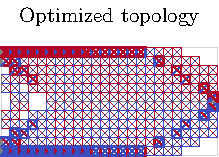
\includegraphics{figures/06_DMO/00_fixed_cells/top_00.pdf}}
    \hfill
    \subcaptionbox{$V = 1567.216$}{\includegraphics{figures/06_DMO/00_fixed_cells/weight_00.pdf}}
    \hfill
    \subcaptionbox{}{\includegraphics[height=3.5cm] {figures/06_DMO/00_fixed_cells/ramp_00.pdf}}
    \hfill
    \subcaptionbox{$V = 8808.671$}{\includegraphics{figures/06_DMO/00_fixed_cells/weight_00_PP.pdf}}
    \bigskip
    \subcaptionbox{}{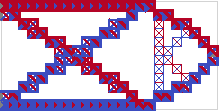
\includegraphics{figures/06_DMO/00_fixed_cells/top.pdf}}
    \hfill
    \subcaptionbox{$V = 1961.175$}{\includegraphics{figures/06_DMO/00_fixed_cells/weight.pdf}}
    \hfill
    \subcaptionbox{}{\includegraphics[height=3.5cm]{figures/06_DMO/00_fixed_cells/ramp.pdf}}
    \hfill
    \subcaptionbox{$V = 3414.214$}{\includegraphics{figures/06_DMO/00_fixed_cells/weight_PP.pdf}}
    \caption{}
    \label{fig:06_fixed_module}
\end{figure*}

To solve this problem, we set up a multi-phase \gls{ramp} interpolation where we simultaneously penalize mechanical properties (using the parameter $p$) and we artificailly icrease the volume (using the parameter $q$) of modules with intermediate weights. In this optimization we set $p=8$ and $q_\text{min}=-0.8$, and a continuation scheme is used on the $q$ parameter to gradually decresase it to the minimum value as already explained in \secref{sec:06_num_app}. The optimized structure topology with penaliized intermediate weights is shown in \figref{fig:06_fixed_module}e and \figref{fig:06_fixed_module}f and it has a volume $V = 1961.175$, a \qty{25}{\percent} volume increase with respect to the unpenalized structure. however we can clearly see how this solution present way less subdomains with intermediate weight and this is very reflected after the thresolding phase shown in \figref{fig:06_fixed_module}h, in wich the volume is now $V=$, more thatn \qty{60}{\percent} less than the unpenalized structure. the difference between the structure of fig and fig could also be less , as in this case we see that the subdomains creates beams tat are made by only an elements and it is enough to transfer the loads. a finer subdivision of the initial structure could then beneficial.

Similarities with classic topology optimization. \sidecite{bendsoe_material_1999,sigmund_non-optimality_2016}

Now that we assessed the need for a penalization scheme, we test the proposed optimization formulation with some test cases using multiple fixed modules. As the topology of the module ($\bar{a}$) is not modified, no perturbation is done on the initial starting point and alpha at iteration 0 is set to $\alpha = 0.5,\,\forall j,t $. First test we performed was to optimize the layout of two different modules ($N_\text{T}$=2) that present the same cell topology connectivity but different cross-sectional areas. we used two 2-nodes fully connected modules with uniform coss sectional areas set to 0.6 and 0.2, to simulate high and low densities modules for hig and low stress part of the structure. The results are presentedi in \figref{fig:06_multiple_fixed}a and b and the structure optimized present a volume $V = 2987.437$. This represent a \qty{12}{\percent} improvement over the single fixed topology.
\begin{figure*}
    \hspace*{\fill}
    \subcaptionbox{}{\includegraphics[height=2.5cm]{figures/06_DMO/00_fixed_cells_multiple/fig1-Topology_area.pdf}}
    \hfill
    \subcaptionbox{$V = 2987.437$}{\includegraphics[height=2.5cm]{figures/06_DMO/00_fixed_cells_multiple/mod_area.pdf}}
    \hspace*{\fill}

    \bigskip

    \hspace*{\fill}
    \subcaptionbox{}{\includegraphics[height=2.5cm]{figures/06_DMO/00_fixed_cells_multiple/fig1-Topology_topol.pdf}}
    \hfill
    \subcaptionbox{$V = 2317.462$}{\includegraphics[height=2.5cm]{figures/06_DMO/00_fixed_cells_multiple/mod_topol.pdf}}
    \hspace*{\fill}
    \caption{}
    \label{fig:06_multiple_fixed}
\end{figure*}

Similar results are presented in \figref{fig:06_multiple_fixed}c and d, in wich we optimize the module layout of two modules that present a different mirrored topology (see \figref{fig:06_multiple_fixed}d). The structure optimized in this way shows a very different module layout and a final volume $V = 2317.462$, even better than before. These two examples confirming that giving more design freedom to the optimizer can improve the mechanical performance of the modular structure. .

\subsection{Modules and layout optimization}
We now optimize a modular structure using multiple modules that can now varry their topology (the values of abar are no fixed nomore). in the case of nt=1, the starting point for the value of alpha is still trivial (alpa=1 forall) and the structure we obtain toghether with the optimized module topology is showed in \figref{fig:06_module_topol_opt}a and b. The modular structure present a volume $V = 2107.983$, the better fuound until this point and confirming the interest in optimizing both the modules topology and layout.
\begin{figure}
    \hspace*{\fill}
    \subcaptionbox{$V = 2107.983$}{\includegraphics[height=2.5cm]{figures/06_DMO/00_optimized_module/fig1-Topology.pdf}}
    \hfill
    \subcaptionbox{}{\includegraphics[width=0.3\linewidth]{figures/06_DMO/00_optimized_module/fig8-Module_Topology_001.pdf}}
    \hspace*{\fill}
    \caption{}
    \label{fig:06_module_topol_opt}
\end{figure}

\begin{figure}
    \centering
    \includegraphics{figures/06_DMO/00_optimized_modules/kmeans.pdf}
    \caption{}
    \label{fig:06_cant_kmeans}
\end{figure}

moving now to the layout and topology optimization of modular structure with a number of module topologies $N_\text{T}$>1,there is the need to use the kmeans clustering to evaluate the strating point for the layout module variable $\alpha$. A \gls{fea} is set up on the original ground structure with uniform cross sectional areasand the kmeans clustering is performed over the stress distribution usinfg $N_\text{T}$ different clusters. The process is shown for example for nt=2 and nt=5 on \figref{fig:06_cant_kmeans}, in wich we see that in general we have the clusters following more and less stressed zones especially in the nt=2 example. But it is only when the number of clusters arrive at 5 that we ctart to see a difference between tension and compression, with a symmetrical solutionn with respect to the asse neutro della trave.

\begin{table}
    \centering
    \small
    \begin{tabular}{lx{1.5cm}x{1.5cm}x{1.5cm}x{1.5cm}x{1.5cm}}
        \toprule
    $N_\text{T}$ & 1&2&3&4&5 \\ \midrule 
    $N_\text{sub}$& 288&288&288&288&288 \\
    $N_\text{sub, e}$ & 107&   45  &   72   &   43   &   50     \\
    $V$  & 2107.983 &  1722.61 &   1730.05  & 1589.90  & 1416.05  \\
    $a_\text{max}$      & 0.37& 0.35  & 0.48  &  0.54  & 0.53   \\
    $\varphi$   &\qty{17.16}{\percent}&\qty{17.86}{\percent}&\qty{14.20}{\percent}&\qty{17.95}{\percent}&\qty{16.65}{\percent}   \\
    $\psi$& 0.52   &  0.59 &  0.57   & 0.61  &0.67      \\
    t        & \hms{0;0;35}  &  \hms{0;0;18} & \hms{0;0;14} & \hms{0;0;17} & \hms{0;0;26}  \\ \bottomrule
    \end{tabular}
    \caption{}
    \label{tab:06_different_topol_cant}
\end{table}
\begin{marginfigure}
        \centering
        \includegraphics[width=\linewidth]{figures/06_DMO/00_multiple_modules_curves/multi_tab.pdf}
        \caption{}
        \label{fig:06_different_topol_cant_crv}
    \end{marginfigure}
Starting form the adviced starting point from the kmeans cludtering, the optimization are performed for nt from 2 to 5, and their results are resumed in the \tabref{tab:06_different_topol_cant}. Here are the main takeawqys :  Having a look at the evolution of the volume of the optimized structures with the different number of modules nt, we notice how they behave like expected as a monotonic descending function. This behaviour could be explained by in general a major specificity of the modules that chan shape their topology to more specific load cases and be less general purpose. We can see effettivamente that the value of the average bar load is increasing with the number of module topologies. This ehaviour is resumed in \figref{fig:06_different_topol_cant_crv}.Additionally it is interesting how, increasing the number of module topologies the number of empty subdomains drop from 107 and stabilize at around 50, suggesting that for this specific test case more modules topologies are employed, the number of empty subdomains decrease, showing that it is better to have many light modules and not few stron and heavy ones. Finally, concerinng the calculation time, we see no real correlation between the number of modules. We speculate that THis is because, even if the number of design variables increase, the problem is often easier  to solve and less iteerations are necessary to attain covergence. The topology of the modular structure with nt=2 e nt=5 is showed togheter whit theri optimized modules in \figref{fig:06_diferent_modules_cant_topology}. It is interesting to notice how the optimized structures shows similar modules layout with respect to the number of module topology.

    \begin{figure*}
        \subcaptionbox{}{\includegraphics[width=0.3\linewidth]{figures/06_DMO/00_optimized_modules/nt2.pdf}}
        \hfill
        \subcaptionbox{}{\includegraphics[width=0.6\linewidth]{figures/06_DMO/00_optimized_modules/nt5.pdf}}
        \caption{}
        \label{fig:06_diferent_modules_cant_topology}
    \end{figure*}



\begin{marginfigure}
    \centering
    \includegraphics[width=\linewidth]{figures/06_DMO/00_optimized_modules/VL/nt=5VL.pdf}
    \caption{$V = 1727.314$}
    \label{fig:06_cant_variable_link}
\end{marginfigure}

last thing we want to comment on is a comparison betweenn the optimized structure with nt=5 of \figref{fig:06_diferent_modules_cant_topology}b and the structure we would obtain if we used the clustering algo suggested structure layout to set the mapping matrix H and the variable linking algorithm described in \secref{sec:05_opt_formulation}. Using this formulation, the layout of the structure is fixed and no changes or empty modules are possible. The optimized structure using this algorithm is shown in \figref{fig:06_cant_variable_link} and it has a volume $V = 1727.314$, more than \qty{20}{\percent} more with respect to the proposed method slution. the differnece can be explained by two factors: forst the proposed formulation permits to have empty subdomains, and this definetly helps for lightening the structure. secondly, the  proposed formulation uses the clustering results only as a starting point for the layout of the optimization, but the layout can then evolve.

\subsection{A benchmark case study: a simply supported modular bridge}
The proposed formulation and solution algorithm is now benchmarked against what we find in the literatre. To the knowledge of the authors, there is no other works that optimize layout and topology of modular structures using a gradient descent algorithm and continuous design variables. However, we can find som similar results obtained using MILP algorithm or simulated annealing to optimize modular structure. This is the case for example of the works of Tugilimana \sidecite{tugilimana_spatial_2017,tugilimana_integrated_2019} and we will now compare the restults. 

\begin{marginfigure}
    \centering
    \includegraphics[width=\linewidth]{figures/06_DMO/00_bailey_bridge/applsci-12-03788-g002.png}
    \caption{Bailey bridge placed on construction site road over Orava river (Slovakia) \cite{prokop_load-carrying_2022}. }
    \label{fig:06_bailey}
\end{marginfigure}

The considered structure is a modular structure based on the Bailey bridge \sidecite{department_of_the_army_bailey_1986}, a concept that has been studied for military puropses and used also for civil applications \eg temporary bridge structures, thanks adaptability, low weight, but especially extremely fast erection and almost immediate usability for traffic are utilized (see \figref{fig:06_bailey}). The structure is 20 modules long and 2 modules high, each module is \qty{3.050}{m} long (\qty{10}{ft}) and \qty{1.525}{m} high (\qty{5}{ft}), resulting in a total bridge span of \qty{30.50}{m} (\qty{100}{ft}). The load case is represented in \figref{fig:06_tug_bcs}, toghether with the geometrical and material data (normalized) used for the optimization in \tabref{tab:06_modular_tug}. We optimize here only the symmetric part. In this load case we consider all the constraints of the formulation \eqrefnotext{} but the buckling, as Tugilimnana did.

\begin{figure}
    \centering
    \includegraphics{figures/06_DMO/00_tug_bench_bcs/bcs.pdf}
    \caption{}
    \label{fig:06_tug_bcs}
\end{figure}

\begin{margintable}
    \small
    \centering
    \begin{tabular}{cc}
    \toprule
    \textbf{Parameter}        & \textbf{Value} \\ \midrule
    $L$              & 3.05     \\
    $\sigma_\text{c}, \sigma_\text{t}$ & $\pm 1$\\
    $P$              & 1   \\
    \bottomrule
    \end{tabular}
    \caption{Material data used for the }
    \label{tab:06_modular_tug}
\end{margintable}

The resulting optimized stuctures are presented in the right part of \figref{fig:00_tug_bench}, toghether with the topology of the structures optimized by Tugilimana \etal \sidecite{tugilimana_integrated_2019}. Below every subfigure it is present the structure voulume and, in square bqrckets, the relative value wwith respect to the Tugilimana solution. Even if the reference images doesnet higlight the submodules that shows the same module topology, we see that the module layout is not always the same \eg in the case of $N_\text{T}=4$ or $N_\text{T}=5$.  We notice tat the proposed optimization algorithm is not only capable of optimizing an intrinsically discrete optimization problem using continuous design variables and a gradient based optimizer, but also to improve the results found in the literature up to \qty{3}{\percent}. The structure obtained with nt=10 is exactly the same we would otain by optimizing the structure if we didnt consider the modular constraints.


\begin{figure*}
    \centering
    \includegraphics{figures/06_DMO/00_tug_bench/bench.pdf}
    \caption{}
    \label{fig:00_tug_bench}
\end{figure*}

Up untill now we used always normalized materila data and dimensions and we never considered local buckling of truss. We test for that reason what happens in this very load case if we do that, and we are very interested in seeing if these changes affects a lot the modules topology and layout in the structure. The material data used for the optim is presented in \tabref{tab:06_modular_tug_buck} and represent an aluminium. The cross sections are supposed circular for the local buckling evaluation. THe topological buckling is taken into account inside the modules as already explained in \secref{sec:05_topological}.

\begin{margintable}
    \small
    \centering
    \begin{tabular}{cc}
    \toprule
    \textbf{Parameter}        & \textbf{Value} \\ \midrule
    $L$              & \qty{3.05}{m}     \\
    $E$              & \qty{69}{GPa}     \\
    $\sigma_\text{c}, \sigma_\text{t}$ & $\pm $\qty{270}{MPa} \\
    $P$              & \qty{1}{MN}   \\
    \bottomrule
    \end{tabular}
    \caption{Material data used for the }
    \label{tab:06_modular_tug_buck}
\end{margintable}

The optimized structure for the Bailey bridge with buckling constraints are shown for a different number of module topologies in \figref{fig:06_tug_bench_buck}. quickly comparing them with the results without the buckling we notice that for this test case the layout of the modules is the same. The topology however is very different with in general a litte bit less active bars. The volume cand be directly compared, so we normalize them and plot them on \figref{fig:06_cant_volume_norm}, showing that adding multiple module topologies is beneficial in the same exact way with or without buckling constaints. We can also comment that the biggest reduction on the volume from the inclusion of additional modules come expecially at the beginning, \eg going from nt=1 to nt=2 or from nt=2 to nt=3, while the difference at higher numbers is marginal as the succession show a plateau.

\begin{marginfigure}
    \centering
    \includegraphics{figures/06_DMO/00_tug_bench_crv/vol.pdf}
    \caption{}
    \label{fig:06_cant_volume_norm}
\end{marginfigure}

\begin{figure}
    \centering
    \includegraphics{figures/06_DMO/00_tug_bench_buck/buck.pdf}
    \caption{}
    \label{fig:06_tug_bench_buck}
\end{figure}

willing to explore how the different parameters can influence the results, the topology and the layout, we test the same load case with a different number of subdomains and modules. We use the very same test case, with the only difference that we are now using a 3x2 nodes ground structure for having faster calculation times. 

\begin{figure*}
    \centering
    \includegraphics{figures/06_DMO/00_tug_bench_size/size.pdf}
    \caption{}
    \label{fig:06}
\end{figure*}
Commenta volume, di come Influence of the number \figref{fig:06_cant_volume_norm_2}
of subdomains on the volume of the steep increase and then plateau, different from before
optimized modular structure cambia e non sale piu in maniera ma si stoppa a un plateau
principalmente due motivi, cambia il metodo di rottura, non piu buckling e passo a stress e poi ho i vuoti. we observe that when we have not many subdomains the structure is always all filled, with  no empty subdomains. but with the increasing number of subdomains we notice more and more empty subdomains, helping to keep the structure light.

\begin{marginfigure}
    \centering
    \includegraphics{figures/06_DMO/00_tug_bench_crv2/vol.pdf}
    \caption{}
    \label{fig:06_cant_volume_norm_2}
\end{marginfigure}

last thing commenta per esempio imm d in cui cambia il modo di rottura e la cell é simmetrica in compressione e in tensione. molto efficace uso del materiale in questa maniera e quindi il volume scende.

\subsection{Simply supported 3D beam}
The last test we conduct is on the simply supported 3d beam, a load case introduced in Chapter~\ref{chap:04} and used tout au long de cette these. we rappel the test case and the material and geometric data used for the optimization process in \figref{fig:06_symm_support_bc} and \tabref{tab:06_3D_supp_mat}.as already done we optimize here onky one forth of the entire structure thanks to its symmetry planes. we conduct the optimization using 6x2x3 subdomains on the X, Y and Z axis respectively and every module is discretized using a 3x3x3 fully connected ground structure ($\bar{n} = 351$). The ooptimization is conducted using three different number of modules, $N_\text{T}$=1,2,3.

\begin{marginfigure}
    \centering
    \includegraphics[width=\linewidth]{figures/06_DMO/00_supported_bc/supported_3D_symm.pdf}
    \caption{Symmetric boundary conditions of the simply supported 3D beam. In gray are the symmetry planes of the test case.}
    \label{fig:06_symm_support_bc} 
\end{marginfigure}

\begin{margintable}
    \small
    \centering
    \begin{tabular}{cc}
    \toprule
    \textbf{Parameter}        & \textbf{Value} \\ \midrule
    $E$              & \qty{2.7}{GPa}     \\
    $\sigma_\text{c}, \sigma_\text{t}$ & $\pm $\qty{55}{MPa} \\
    $\rho$              & \qty{1.14}{\gram\per\cubic\centi\metre}   \\
    $P$              & \qty{100}{N}   \\
    \bottomrule
    \end{tabular}
    \caption{Material data used for the simply supported 3D beam optimization.}
    \label{tab:06_3D_supp_mat}
\end{margintable}

The resulting optimized structures are presented in \figref{fig:06_supp_top} and the associated numerical results are presented in \tabref{tab:06_supp_tab}. The first thing we notice is that in this specific test case the optimizer converges to solutions where the sum of alpha for every subdomains is always equal to one. whyle before we have seen that the formulation arrived at create empty subdomains where the sum of alpha is zero, here the optimizer failed. the empty subdomains of the nt=2 and nt=3 corresponds to cases where the topology of one module is set to zero and the optimizer put thee value of the corresponding alpha to one. In this way the solution is still optimized correctly, but using a module topology en plus \eg looging at \figref{fig:06_supp_top}b and e, so the solution for nt=2, we see that the optimized structure shows only one module topology, the other being the empty one.

we speculate that this problem come from the optimizer's settings used to normalize the design variables and the constraint for the opmimization. we found that for example even if we scaled the alpha variable and the corresponding constraints in multiple values, we still got the same results. THis problem suggest us that even if the starting point perturbation definetly helps achieving a good optiized structure, more work has to be done on developing a new resolution strategy, maybe trying to separate thethe topology and layout varaiables and solving iteratively the two problem separated one iteration at a time.

Even having this problem we can however notice having a look at the volume $V$ and the mean densities $\bar{\rho}$ of \tabref{tab:06_supp_tab} how the modular structures with nt=2 and nt=3 reaches very similar values to the monolitich reference ($n_sub=1$) shown in \figref{fig:06_supp_ref}, while beeing modular.

\begin{figure*}
    \hspace*{\fill}
    \subcaptionbox{}{\includegraphics[width=0.30\linewidth]{figures/06_DMO/00_print_topology/1_04_Topology_NLP_iso.png}}
    \hfill
    \subcaptionbox{}{\includegraphics[width=0.30\linewidth]{figures/06_DMO/00_print_topology/2_04_Topology_NLP_iso.png}}
    \hfill
    \subcaptionbox{}{\includegraphics[width=0.30\linewidth]{figures/06_DMO/00_print_topology/3_04_Topology_NLP_iso.png}}
    \hspace*{\fill}
    \bigskip
    \hspace*{\fill}
    \subcaptionbox{}{\includegraphics[width=0.30\linewidth]{figures/06_DMO/00_print_topology/1_04_Topology_NLP_XZ.png}}
    \hfill
    \subcaptionbox{}{\includegraphics[width=0.30\linewidth]{figures/06_DMO/00_print_topology/2_04_Topology_NLP_XZ.png}}
    \hfill
    \subcaptionbox{}{\includegraphics[width=0.30\linewidth]{figures/06_DMO/00_print_topology/3_04_Topology_NLP_XZ.png}}
    \hspace*{\fill}
    \caption{}
    \label{fig:06_supp_top}
\end{figure*}

\begin{table}
    \centering
    \small
    \begin{tabular}{lx{1.8cm}x{1.8cm}x{1.8cm}x{1.8cm}}
        \toprule
    $N_\text{T}$ & --     & 1     &  2    &  3  \\ \midrule
    $N_\text{sub}$           &    1  &   36   &   36   &   36     \\
    $N_\text{opt}\;(N_\text{el})$  &  20 (1984) &  360 (12636)   &  204 (12636)   &  104 (12636)        \\
    $V$ [\unit{cm^3}] & 9.907 &  27.958 &   15.548  & 10.178    \\
    $V$ [\unit{\percent}] & 1.761 & 4.970&2.764 & 1.809    \\
    $\bar{\rho}$ [\unit{kg/m^3}] & 80.31 &226.65 &126.05 &82.51 \\
    C [\unit{J}]      &  3.71  &  5.20   &  6.21  & 4.141  \\
    $a_\text{max}$ [\unit{mm^2}]      & 37.61& 9.40  & 12.81  &   15.81     \\
    $\varphi$   &\qty{100.00}{\percent}&\qty{21.11}{\percent}&\qty{39.21}{\percent}&\qty{80.77}{\percent}  \\
    $\psi$& 1.00   &  0.47 &  0.66   & 0.87        \\
    t        & \hms{0;0;4}  &  \hms{0;1;18} & \hms{0;0;42} & \hms{0;10;22}   \\ \bottomrule
    \end{tabular}
    \caption{}
    \label{tab:06_supp_tab}
    \end{table}

    \begin{marginfigure}
        \centering
        \includegraphics[width=\linewidth]{figures/04_TTO_improvements/16_supported_3D_sol/04_Topology_NLP_iso-min.png}
        \caption{Perspective view of the monolithic simply supported 3D beam optimized structure with $V=\qty{9.907}{\centi\meter^3}$}
        \label{fig:06_supp_ref}
    \end{marginfigure}

\section{Conclusion}
in this chapter we presented an innovative optimization formulation that optimize the structural volume of modular structures. The solving algorithm takes advantages of the physical informations of the model, exploiting the analitical derivatives, and uses a gradient descent optimization algorithm. The discrete cathegorical variables used to choose the module layout are modelized using a weighted sum of cotinuous weights, that fits the optimization scheme, and a double penalization scheme is proposed to reduce the appearance of non physical interemediate weights. The proposed formulation is testet over a multitude of test cases, two and three dimensional, from the literature or innovative.these test assessed that the use of this optimization formulation helps the modular structures to achieve volumes that are really near the ones from monolithic optimization, all being modular, offering a good tradeoff between optimality and manufacturing complexity. However, up untill now we concentrated only on dummy test cases that are not of an engineering relevance. for that reason, in the next chapter we address this problem by focussing on the application of the presented optimization formulations in the aerospace context. 